\documentclass[a4paper,twocolumn]{article} % Document type

\ifx\pdfoutput\undefined
    %Use old Latex if PDFLatex does not work
   \usepackage[dvips]{graphicx}% To get graphics working
   \DeclareGraphicsExtensions{.eps} % Encapsulated PostScript
 \else
    %Use PDFLatex
   \usepackage[pdftex]{graphicx}% To get graphics working
   \DeclareGraphicsExtensions{.pdf,.jpg,.png,.mps} % Portable Document Format, Joint Photographic Experts Group, Portable Network Graphics, MetaPost
   \pdfcompresslevel=9
\fi
\usepackage{multirow}
\usepackage{subcaption}
\usepackage{amsmath,amssymb}   % Contains mathematical symbols
\usepackage[ansinew]{inputenc} % Input encoding, identical to Windows 1252
\usepackage[english]{babel}    % Language
%\usepackage[round,authoryear]{natbib}  %Nice author (year) citations
\usepackage[square,numbers]{natbib}     %Nice numbered citations
%\bibliographystyle{unsrtnat}           %Unsorted bibliography
\bibliographystyle{plainnat}            %Sorted bibliography

\addtolength{\topmargin}{-30mm}% Removes 30mm from the top margin
\addtolength{\textheight}{30mm}% Adds it to the text height


\begin{document}               % Begins the document

\title{Reproducing Sequential Attention for Feature Selection}
\author{Gary Wang, Hank Lai \\ N16132087, N16132079 \\ n16132087@gs.ncku.edu.tw, n16132079@gs.ncku.edu.tw} 
%\date{2010-10-10}             % If you want to set the date yourself.

\maketitle                     % Generates the title




%%%%%%%%%%%%%%%%%%%%%%%%%%%%%%%%%%%%%%%%%%%%%%%%%%%%%%%%%%%%%%%%%%%%%%%%%%%%%%%%%%%
% Instructions regarding the report
%%%%%%%%%%%%%%%%%%%%%%%%%%%%%%%%%%%%%%%%%%%%%%%%%%%%%%%%%%%%%%%%%%%%%%%%%%%%%%%%%%%

\section{Introduction}

Feature selection is essential for improving interpretability, generalization, and efficiency in high-dimensional learning tasks.
 However, As noted in a review by Nordling (2013, Chapter 5.2) have noted, it remains a challenging problem due to 
computational limits and sensitivity to noise. Classical methods such as LASSO and greedy search either fail to capture feature interactions or lack robustness.

Sequential Attention (SA)~\cite{yasuda2023} proposes a novel attention-based relaxation of greedy selection that models conditional importance adaptively. 
In this study, we aim to reproduce SA and evaluate whether it consistently outperforms classical methods 
like Sequential LASSO and Group LASSO.


\section{Methods}
%\subsection{Sequential Attention Algorithm}
% Description of algorithm, possibly Algorithm 1 from paper

\subsection{Experimental Setup}
% Dataset info, network architecture, optimizer, seeds, etc.
In our experimental setup, we utilized the official GitHub repository provided by the original authors to reproduce Figure 3 from the paper. All hyperparameter settings(including model architecture, learning rate, batch size, number of epochs, and other configurations) were kept identical to those reported in the original paper to ensure reproducibility and fair comparison.

\section{Results}
\subsection{ Small-scale experiments}
Small-scale experiments evaluate feature selection methods on benchmark datasets using a simple neural network with 50 selected features.
\subsubsection{Visuallization Of Selected MNIST Features}

In Figure~\ref{fig:feature_masks}, we extracted reference feature maps from the original paper and converted them into binary masks. To select a representative reference mask for comparison, we computed the Structural Similarity Index (SSIM) between each reference candidate and our reproduced results, and chose the one with the highest SSIM as the basis for subsequent comparison.

\begin{figure*}[h!]
    \centering
    % Top row: Reference
    \begin{subfigure}[t]{0.19\linewidth}
        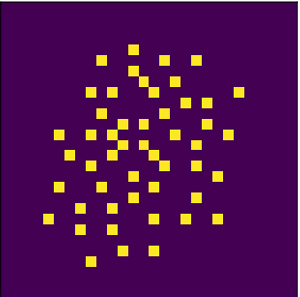
\includegraphics[width=\linewidth]{figures/reference_features_sa.png}
    \end{subfigure}
    \hfill
    \begin{subfigure}[t]{0.19\linewidth}
        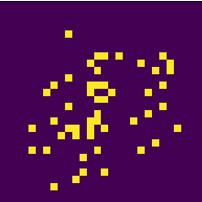
\includegraphics[width=\linewidth]{figures/reference_features_lly.png}
    \end{subfigure}
    \hfill
    \begin{subfigure}[t]{0.19\linewidth}
        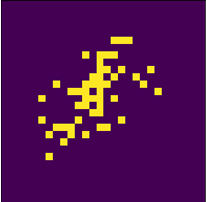
\includegraphics[width=\linewidth]{figures/reference_features_gl.png}
    \end{subfigure}
    \hfill
    \begin{subfigure}[t]{0.19\linewidth}
        
\includegraphics[width=\linewidth]{figures/reference_features_seql.png}
    \end{subfigure}
    \hfill
    \begin{subfigure}[t]{0.19\linewidth}
        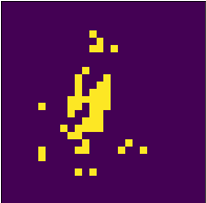
\includegraphics[width=\linewidth]{figures/reference_features_omp.png}
    \end{subfigure}

    \vspace{1em}

    % Bottom row: Best Seeds
    \begin{subfigure}[t]{0.19\linewidth}
        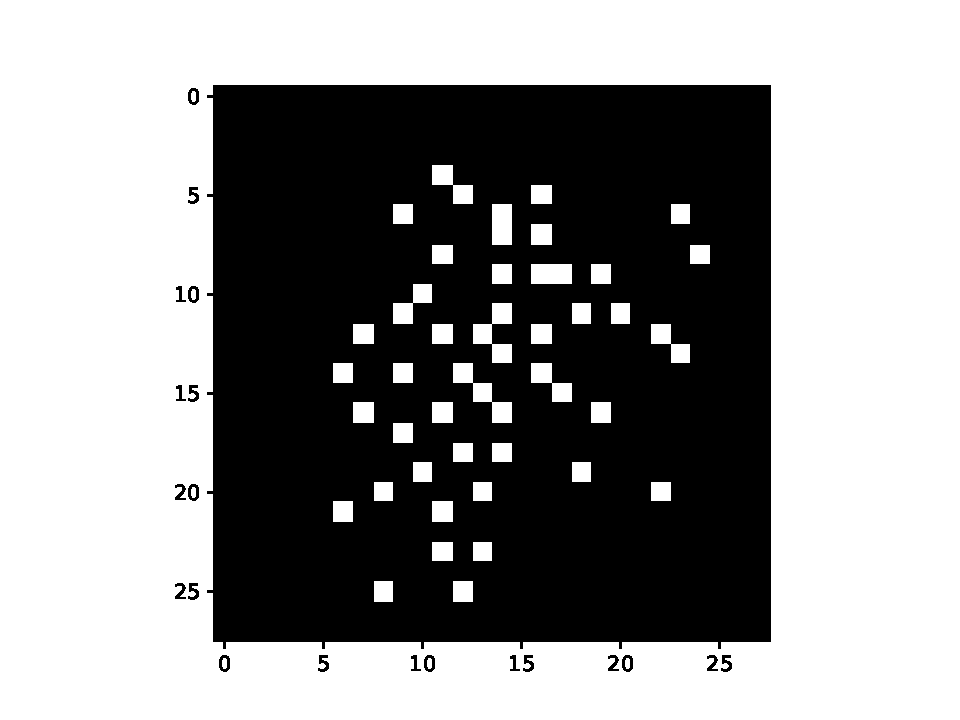
\includegraphics[width=\linewidth]{figures/best_seed_sa.pdf}
    \end{subfigure}
    \hfill
    \begin{subfigure}[t]{0.19\linewidth}
        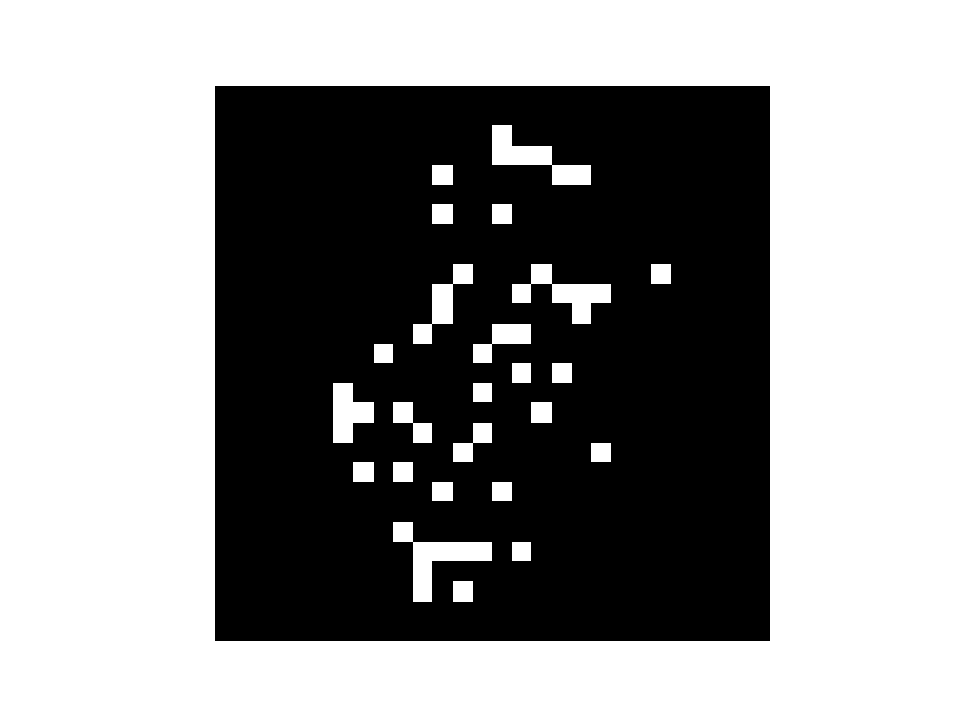
\includegraphics[width=\linewidth]{figures/best_seed_lly.pdf}
    \end{subfigure}
    \hfill
    \begin{subfigure}[t]{0.19\linewidth}
        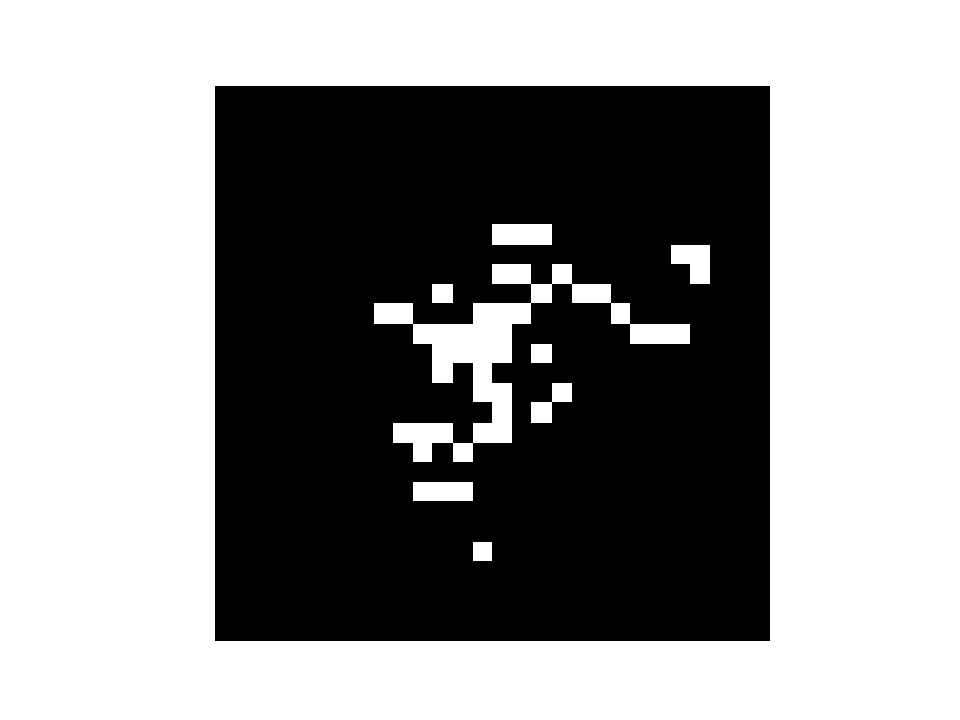
\includegraphics[width=\linewidth]{figures/best_seed_gl.pdf}
    \end{subfigure}
    \hfill
    \begin{subfigure}[t]{0.19\linewidth}
        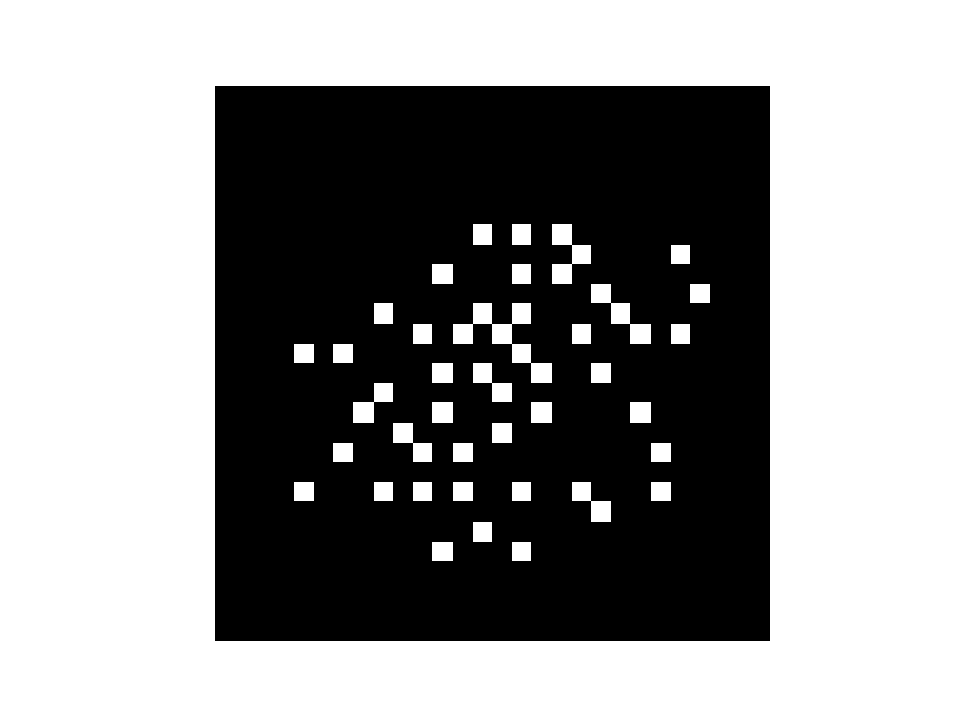
\includegraphics[width=\linewidth]{figures/best_seed_seql.pdf}
    \end{subfigure}
    \hfill
    \begin{subfigure}[t]{0.19\linewidth}
        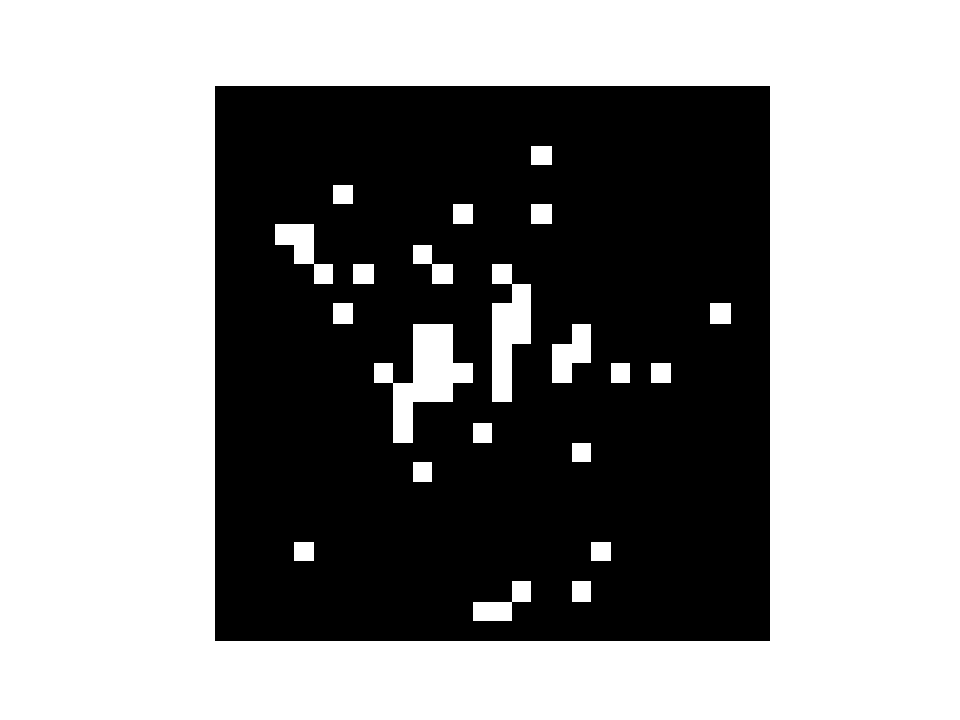
\includegraphics[width=\linewidth]{figures/best_seed_omp.pdf}
    \end{subfigure}

    \caption{Top row: reference masks; bottom row: best-seed selection results for each method.}
    \label{fig:feature_masks}
\end{figure*}


\begin{table}[ht]
    \centering
    \begin{tabular}{lcc}
        \hline
        \textbf{Method} & \textbf{Seed} & \textbf{SSIM} \\
        \hline
        SA    & 3 & 0.0992 \\
        GL    & 5 & 0.3249 \\
        OMP   & 1 & 0.1401 \\
        SEQL  & 2 & 0.0874 \\
        \hline
    \end{tabular}
    \caption{SSIM values for the best seed selected by each method.}
    \label{tab:ssim_results}
\end{table}
%\subsection{Dataset Overview}


\subsubsection{Feature Selection Accuracy}
% Accuracy table or plots for k=50 features
\subsubsection{Statistical Validation}
% t-test or p-value results table if needed
\begin{table}[ht]
\centering
\scriptsize
\begin{tabular}{lccccc}
\hline
\textbf{Dataset} & \textbf{SA} & \textbf{LLY} & \textbf{GL} & \textbf{SL} & \textbf{OMP} \\
\hline
Mice     & 0.9276 & 0.0220 & 0.0227 & 0.0673 & 0.5906 \\
MNIST    & 0.0961 & 0.0013 & 0.0002 & 0.0000 & 0.0607 \\
Fashion  & 0.0105 & 0.8313 & 0.0031 & 0.0007 & 0.0000 \\
ISOLET   & 0.0551 & 0.6804 & 0.0003 & 0.3600 & 0.0037 \\
COIL-20  & 0.3895 & 0.5901 & 0.0093 & 0.1437 & 0.3519 \\
Activity & 0.7448 & 0.3194 & 0.7802 & 0.0034 & 0.2388 \\
\hline
\end{tabular}
\caption{p-values comparing our reproduction results with paper baselines.}
\label{tab:pvalue-comparison}
\end{table}


\begin{table*}[ht]
\centering
\resizebox{\textwidth}{!}{
\begin{tabular}{lccccc}
\hline
\textbf{Dataset} & \textbf{Our results} & \textbf{Lemhadri (2021)~\cite{lemhadri2021lassonet}} & \textbf{p-value} & \textbf{Yasuda (2023)} & \textbf{p-value} \\
\hline
Mice Protein     & 0.989 $ \pm $ 0.008 & 0.990 & 0.7623 & 0.963 & 0.0017 \\
MNIST            & 0.973 $ \pm $ 0.001 & 0.928 & 0.0000 & 0.953 & 0.0000 \\
MNIST-Fashion    & 0.874 $ \pm $ 0.003 & 0.833 & 0.0000 & 0.869 & 0.0297 \\
ISOLET           & 0.950 $ \pm $ 0.003 & 0.953 & 0.1269 & 0.961 & 0.0015 \\
COIL-20          & 0.994 $ \pm $ 0.002 & 0.996 & 0.1381 & 0.986 & 0.0005 \\
Activity         & 0.942 $ \pm $ 0.002 & 0.853 & 0.0000 & 0.954 & 0.0002 \\
\hline
\end{tabular}
}
\caption{Comparison of accuracy using all features. p-values are from one-sample t-tests against Lemhadri et al. and Yasuda et al.'s reported means.}
\label{tab:all-feature-pval}
\end{table*}
\begin{table*}[ht]
\centering
\resizebox{\textwidth}{!}{%
\begin{tabular}{llcccccc}
\hline
\textbf{Dataset} &  & \textbf{SA} & \textbf{LLY} & \textbf{GL} & \textbf{SL} & \textbf{OMP} & \textbf{CAE} \\
\hline
\multirow{2}{*}{MNIST} &
\textit{Paper} & 
0.956 $\pm$ 0.002 & 0.944 $\pm$ 0.001 & 0.937 $\pm$ 0.003 & 0.959 $\pm$ 0.001 & 0.912 $\pm$ 0.004 & 0.909 $\pm$ 0.007 \\
& \textit{Ours} & 
0.954 $\pm$ 0.001 & 0.938 $\pm$ 0.002 & 0.926 $\pm$ 0.003 & 0.952 $\pm$ 0.001 & 0.892 $\pm$ 0.018 & -- \\
\hline
\multirow{2}{*}{MNIST-Fashion} &
\textit{Paper} & 
0.854 $\pm$ 0.003 & 0.843 $\pm$ 0.005 & 0.834 $\pm$ 0.004 & 0.854 $\pm$ 0.003 & 0.829 $\pm$ 0.008 & 0.839 $\pm$ 0.003 \\
& \textit{Ours} & 
0.846 $\pm$ 0.004 & 0.844 $\pm$ 0.004 & 0.842 $\pm$ 0.003 & 0.845 $\pm$ 0.003 & 0.768 $\pm$ 0.012 & -- \\
\hline
\multirow{2}{*}{ISOLET} &
\textit{Paper} & 
0.920 $\pm$ 0.006 & 0.866 $\pm$ 0.012 & 0.906 $\pm$ 0.006 & 0.920 $\pm$ 0.003 & 0.727 $\pm$ 0.026 & 0.893 $\pm$ 0.011 \\
& \textit{Ours} & 
0.927 $\pm$ 0.005 & 0.869 $\pm$ 0.010 & 0.887 $\pm$ 0.005 & 0.923 $\pm$ 0.007 & 0.808 $\pm$ 0.035 & -- \\
\hline
\multirow{2}{*}{COIL-20} &
\textit{Paper} & 
0.997 $\pm$ 0.001 & 0.994 $\pm$ 0.002 & 0.997 $\pm$ 0.004 & 0.988 $\pm$ 0.005 & 0.967 $\pm$ 0.014 & 0.972 $\pm$ 0.007 \\
& \textit{Ours} & 
0.994 $\pm$ 0.008 & 0.992 $\pm$ 0.006 & 0.991 $\pm$ 0.002 & 0.992 $\pm$ 0.005 & 0.976 $\pm$ 0.016 & -- \\
\hline
\multirow{2}{*}{Activity} &
\textit{Paper} & 
0.931 $\pm$ 0.004 & 0.897 $\pm$ 0.025 & 0.933 $\pm$ 0.002 & 0.931 $\pm$ 0.003 & 0.905 $\pm$ 0.013 & 0.921 $\pm$ 0.001 \\
& \textit{Ours} & 
0.930 $\pm$ 0.003 & 0.908 $\pm$ 0.010 & 0.934 $\pm$ 0.008 & 0.917 $\pm$ 0.006 & 0.887 $\pm$ 0.029 & -- \\
\hline
\multirow{2}{*}{Mice Protein} &
\textit{Paper} & 
0.993 $\pm$ 0.008 & 0.981 $\pm$ 0.005 & 0.985 $\pm$ 0.005 & 0.984 $\pm$ 0.008 & 0.994 $\pm$ 0.008 & 0.956 $\pm$ 0.012 \\
& \textit{Ours} & 
0.993 $\pm$ 0.008 & 0.992 $\pm$ 0.007 & 0.994 $\pm$ 0.006 & 0.994 $\pm$ 0.008 & 0.992 $\pm$ 0.007 & -- \\
\hline
\end{tabular}
}
\caption{Accuracy comparison: paper-reported (top) vs. reproduced results (bottom) across all datasets.}
\label{tab:accuracy-ours-vs-paper}
\end{table*}




\section{Discussion}
% Analysis of differences, strengths, weaknesses, generalization, possible error sources


\subsection{ Large-scale experiments}
We encountered difficulties reproducing the large-scale experiment presented in Figure 4 of the original paper. Specifically, the Criteo Click dataset used in that experiment requires approximately 1TB of disk space. 
Due to hardware limitations on both our local machines and available servers, we were unable to process and store the full dataset. 
As a result, we were not able to reproduce the large-scale results associated with this figure.

\section{Conclusion}
% Summary of what was reproduced and whether claims hold

\bibliographystyle{ieeetr}
\bibliography{references}


% Optionally include appendix
\clearpage
\appendix
\section*{Appendix}
\section{Hyperparameters}
% Learning rate, batch size, etc.

\section{Additional Figures}
% Supplementary plots

\end{document}      % End of the document
